\documentclass[tikz]{standalone}
% ------- TikZ Preamble -------
\RequirePackage{tikz}

\usetikzlibrary{
    spath3,
    intersections,
    arrows,
    knots,
    calc,
    hobby,
    decorations.pathreplacing,
    shapes.geometric,
     decorations.markings,
    decorations.pathmorphing,
    tikzlings}

% ------- Shared styles (from your preamble) -------
\tikzset{
    knot diagram/every strand/.append style={ultra thick, black},
%               every path/.style={black,line width=2pt},
%               every node/.style={transform shape,knot crossing,inner sep=1.5pt},
%               every knot/.style={line cap=round,line join=round,very thick},
%               strand/.style={line cap=round,line join=round,line width=3pt,draw=black},
%               over/.style={preaction={draw=white,line width=6.5pt}},
%               sst/ring A/.style={draw=black, line width=3pt},
%               sst/ring B/.style={draw=black,  line width=3pt},
%               sst/ring C/.style={draw=black, line width=3pt},
}
\begin{document}
%=============================================================================

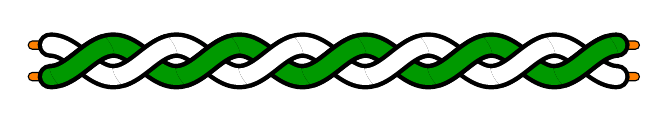
\begin{tikzpicture}[fat line/.style={black, double=#1,double
distance=6pt,looseness=1.2,line cap=round}]
\begin{knot}[%draft mode = crossings, % uncomment to see where the crossings are
clip width = 0,
flip crossing/.list={1,3,5,7,9}]
\path foreach \X in {0,4.5} {foreach \Y in {0.2,-0.2}
{(1.6*\X,\Y) node[draw,fill=orange,inner ysep=1.5pt,inner xsep=8pt,rounded
corners=1.5pt]{}}};
\strand[fat line=white]
     plot[domain=0:4.5,samples=251] (1.6*\x,{0.2*cos(\x*360)});
\strand[fat line=green!60!black]
   plot[domain=0:4.5,samples=251] (1.6*\x,{-0.2*cos(\x*360)});
\end{knot}
\end{tikzpicture}
%=============================================================================

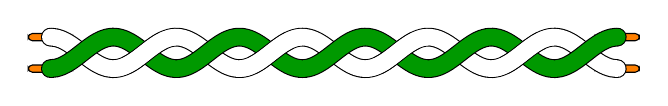
\begin{tikzpicture}[fat line/.style={black, double=#1,double
distance=6pt,looseness=1.2,line cap=round}]
\path foreach \X in {0,4.5} {foreach \Y in {0.2,-0.2}
{(1.6*\X,\Y) node[draw,fill=orange,inner ysep=1.3pt,inner xsep=8pt,rounded
corners=1.5pt]{}}};
\draw[fat line=white]
     plot[domain=0:4.5,samples=101,smooth] (1.6*\x,{0.2*cos(\x*360)});
\draw[fat line=green!60!black]
   plot[domain=0:4.5,samples=101,smooth] (1.6*\x,{-0.2*cos(\x*360)});
\draw[fat line=white,line cap=butt]
 foreach \X in {1,...,4}
 {plot[domain=\X-0.4:\X-0.1,samples=7,smooth] (1.6*\x,{0.2*cos(\x*360)})};
\draw[white,line width=6pt]
 foreach \X in {1,...,4}
 {plot[domain=\X-0.5:\X,samples=11,smooth] (1.6*\x,{0.2*cos(\x*360)})};
\end{tikzpicture}
%=============================================================================


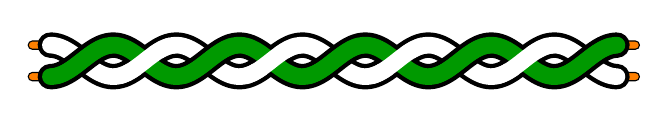
\begin{tikzpicture}[
  basic strand/.style={
    double=.,
    draw=black,
    looseness=1.2,
    double distance=6pt,
    line cap=round
  },
  crossing strand/.style={
    line width=6.8pt,
    only when rendering/.style={%
      draw=\pgfinnerstrokecolor,%
      line width=6pt,
      double=none,
    }
  }
]
\begin{knot}[%draft mode = crossings, % uncomment to see where the crossings are
  clip width = 1,
  flip crossing/.list={1,3,5,7,9},
  background color=black,
  only when rendering/.style={%
    basic strand
  },%
  every intersection/.style={
    crossing strand
  },
]
\path foreach \X in {0,4.5} {foreach \Y in {0.2,-0.2}
{(1.6*\X,\Y) node[draw,fill=orange,inner ysep=1.5pt,inner xsep=8pt,rounded
corners=1.5pt]{}}};
\strand[white]
     plot[domain=0:4.5,samples=251] (1.6*\x,{0.2*cos(\x*360)});
\strand[green!60!black]
   plot[domain=0:4.5,samples=251] (1.6*\x,{-0.2*cos(\x*360)});
\end{knot}
\end{tikzpicture}

%=============================================================================


    \tikzset{
        fat line/.style={black,double=#1,double distance=6pt,line cap=round}
    }
    \begin{tikzpicture}
        \draw[fat line=white]
            plot[domain=0:4.5,samples=101,smooth](1.6*\x,{0.2*cos(\x*360)});
        \draw[fat line=green!60!black]
            plot[domain=0:4.5,samples=101,smooth](1.6*\x,{-0.2*cos(\x*360)});
        % change yellow to white
        \draw[fat line=yellow,cap=butt,dash pattern=on20off32,dash phase=-1]
            plot[domain=0:4.5,samples=101,smooth](1.6*\x,{0.2*cos(\x*360)});
        % un-comment for even better clipping effect
        %\draw[white,line width=6,cap=butt,dash pattern=on24off28,dash phase=1]
        %   plot[domain=0:4.5,samples=101,smooth](1.6*\x,{0.2*cos(\x*360)});
    \end{tikzpicture}






\end{document}

